\chapter{Numerical Calculations}
\newcommand{\lso}{\ensuremath{L_{\textnormal{SO}}}}
\newcommand{\tso}{\ensuremath{t_{\textnormal{SO}}}}

Numerical transport calculations have a huge advantage over the analytical
calculation: once a formalism is implemented, it works for arbitrary
configurations within the limits of the model. However it doesn't generally
supply us with data that enhances physical understanding, so its best use as a
means to expand on analytical calculations which we already understand.

In that spirit we performed numeric calculations, simulating a sample with
Rashba Spin-orbit coupling, and spin-resolved leads attached at the edges.

The calculation follows this rough scheme:

\begin{itemize}
    \item Set up the Hamiltonian $H$
    \item Calculate the self-energy matrices $\Sigma_p$
    \item Calculate the Green's functions $G^A$ and $G^R$ by inverting
          $H + \sum_p \Sigma_p$
    \item Use the Fisher-Lee relation to calculate the transmission matrix $T$
            from $G^R$, $G^A$ and $\Sigma_p$
\end{itemize}

\section{Performance consideration}

These numeric calculations are computationally expensive. If we simulate a
lattice with a total of $n \times n$ sites, the matrices $H$, $\Sigma_p$, $G^R$ and
$G^A$ are of dimensions $2n^2 \times 2n^2$. Inversion of an $m \times m $
matrix and multiplication of two $ m \times m $ matrices both take $O(m^3)$
steps\footnote{There are matrix product algorithms with slightly better
asymptotic scaling, but they are usually very complicated, numerically badly
conditioned, or only advantageous for huge systems; usually all three apply}
\cite{matrixperformance}. All other steps are faster, and can be ignored for
an asymptotic analysis.

So the naive approach takes $O(n^6)$ steps for $n \times n$ lattice sites.

An alternative approach, the \emph{Recursive Green's Function method} works by
decomposing the sample into slices in such a way that the sites in each slice
only interact with neighbor slices. For short range interactions such a
decomposition can be found, and for nearest-neighbor hopping the time
complexity approaches $O(n^3)$ \cite{rgfschmelcher}. However this is payed by
a significantly increased implementation complexity, and the algorithm is tied
to the specific form of the Hamiltonian.

\begin{figure}
    \begin{center}
    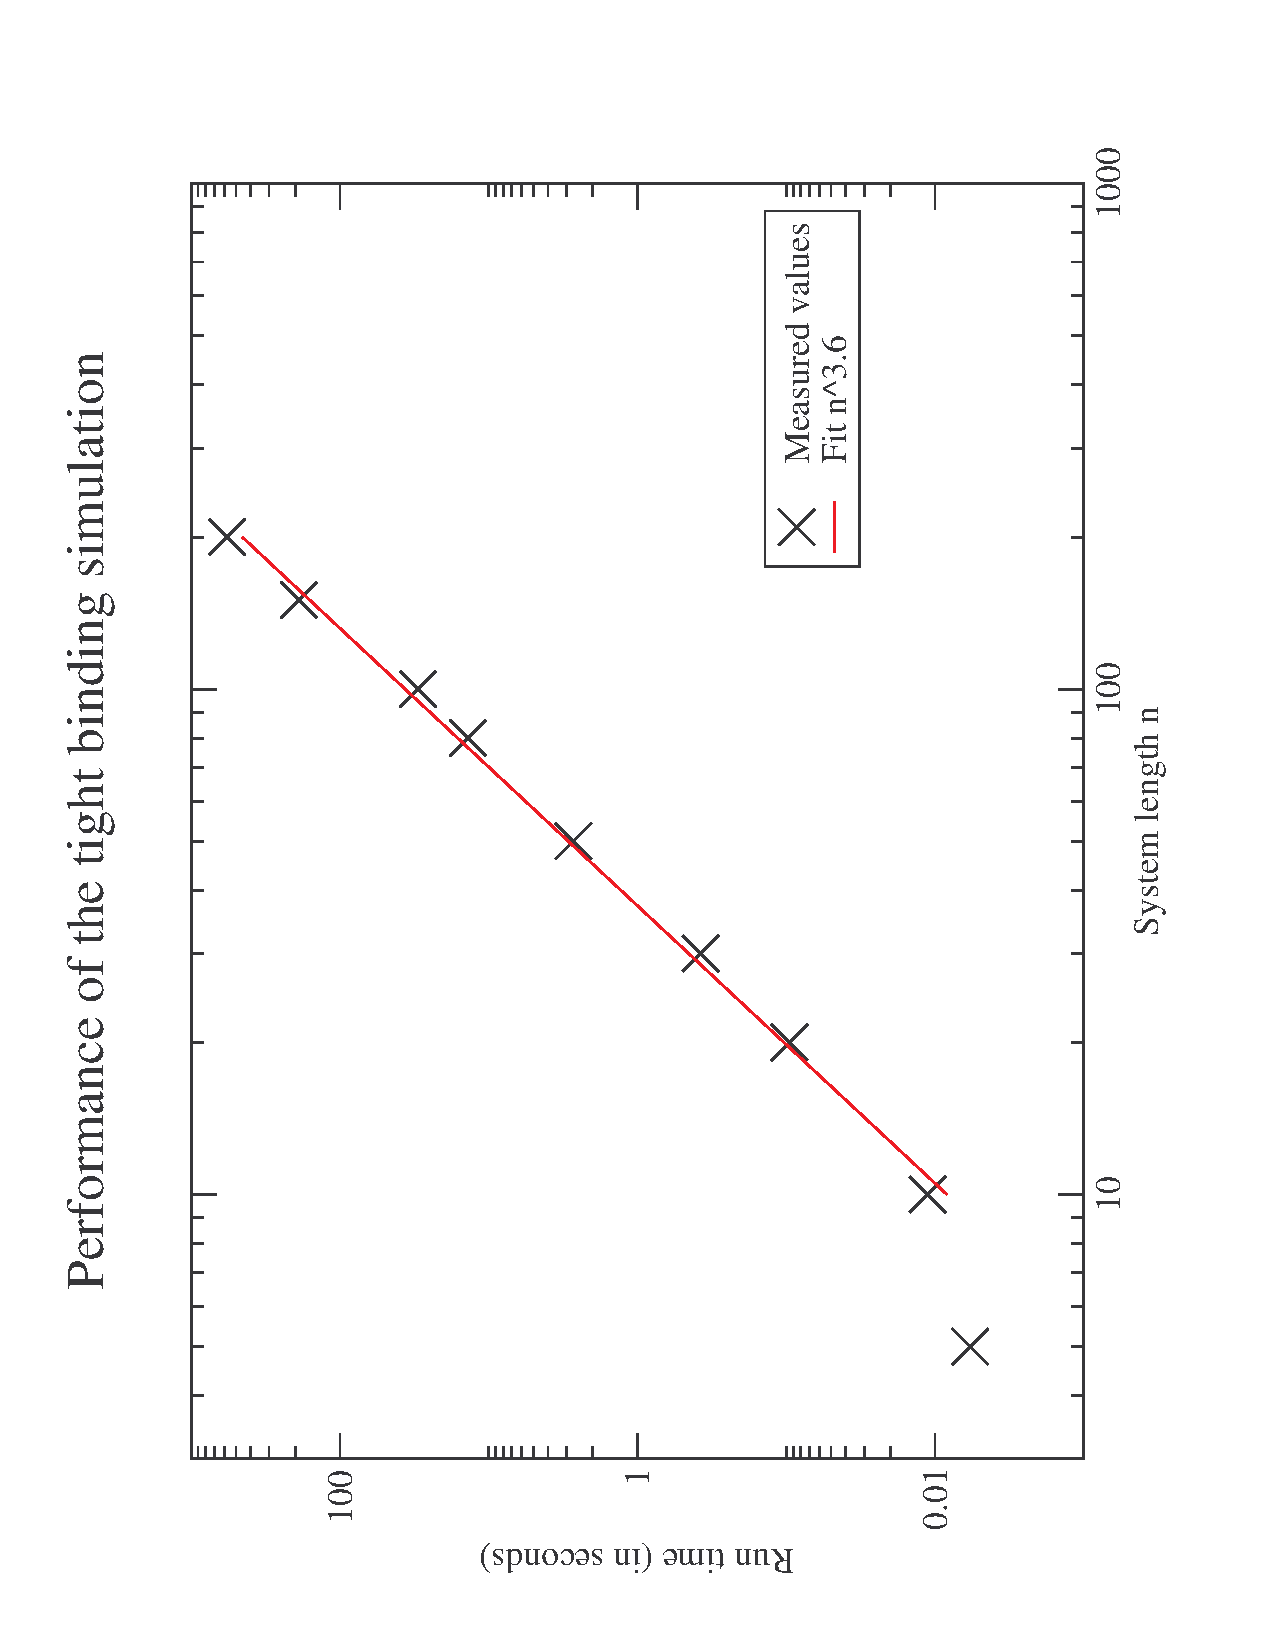
\includegraphics[angle=270,width=0.7\textwidth]{scaling.pdf}
    \end{center}
    \caption{Scaling of run time with system size for the tight binding
        simulation, implemented with sparse matrices and the SuperLU sparse
        direct solver. The data was recorded for square samples including
        Rashba spin-orbit coupling, and 4 leads of the same width as the
        sample, on a 2.9GHz AMD64 computer with SSE2 and 8GB RAM.
        The run time approximately scales as $t(n) = 2
        n^{3.64}\mu s$}
        \label{fig:scaling}
\end{figure}

We chose a middle ground: the "naive" approach, but implemented with sparse
matrices, and using an efficient sparse direct solver\cite{superlu99} for
computing the Green's functions.

The run time thus depends largely on the number of non-zeros in the $H$ and
$\Sigma_p$, and thus on the nature of the interaction. For nearest neighbor
hopping and Rashba spin-orbit coupling we observed a run time scaling of
$O(n^{3.64})$ (See Fig. \ref{fig:scaling}).

\section{Numerical stability}

The numerical
calculation uses floating point numbers with limited machine precision,
therefore numerical errors are inevitable.

The transmission matrix for a sample which is connected to multiple uniform
leads (with same number of modes per lead) has to fulfill the sum rules

\begin{align}
    \sum_p T_{pq} = \sum_q T_{pq} = M
    \label{eq:sumrule}
\end{align}

Where $M$ is the number of modes (and thusly and integer). We can calculate
this left hand side of this equation from the numerical simulation, round it
to the nearest integer and thus estimate the numerical error in $T_{pq}$.

Since generally matrix inversion is numerically worse conditioned than solving
a linear equation system\cite{matrixinversion}, we don't actually compute
$G^A$ and $G^R$, but rather the products $G^A\Sigma_p$ and $G^R\Sigma_q$,
which can be written as solutions of linear equation systems.

\begin{align}
    X_p &= \Sigma_p G^R\\
    X_p^\dagger &= (G^R)^\dagger \Sigma_p^\dagger = G^A \sigma_p^\dagger\\
    \Rightarrow\quad (G^A)^-1 X_p^\dagger &= \Sigma_p^\dagger
    \label{eq:lin_gls}
\end{align}

Eq. \ref{eq:lin_gls} is the form with which linear sparse solvers typically
work. They typically calculate a LU decomposition (that is they write
$(G^A)^-1 = L \cdot U$, where $L$ is a lower triangular matrix and $U$ an
upper triangular matrix), and directly solve the equation by elimination.
Complex conjugation and transposition of $X_p^\dagger$ finally gives us the
matrix which we need evaluating the Fischer-Lee relation.

\begin{figure}
    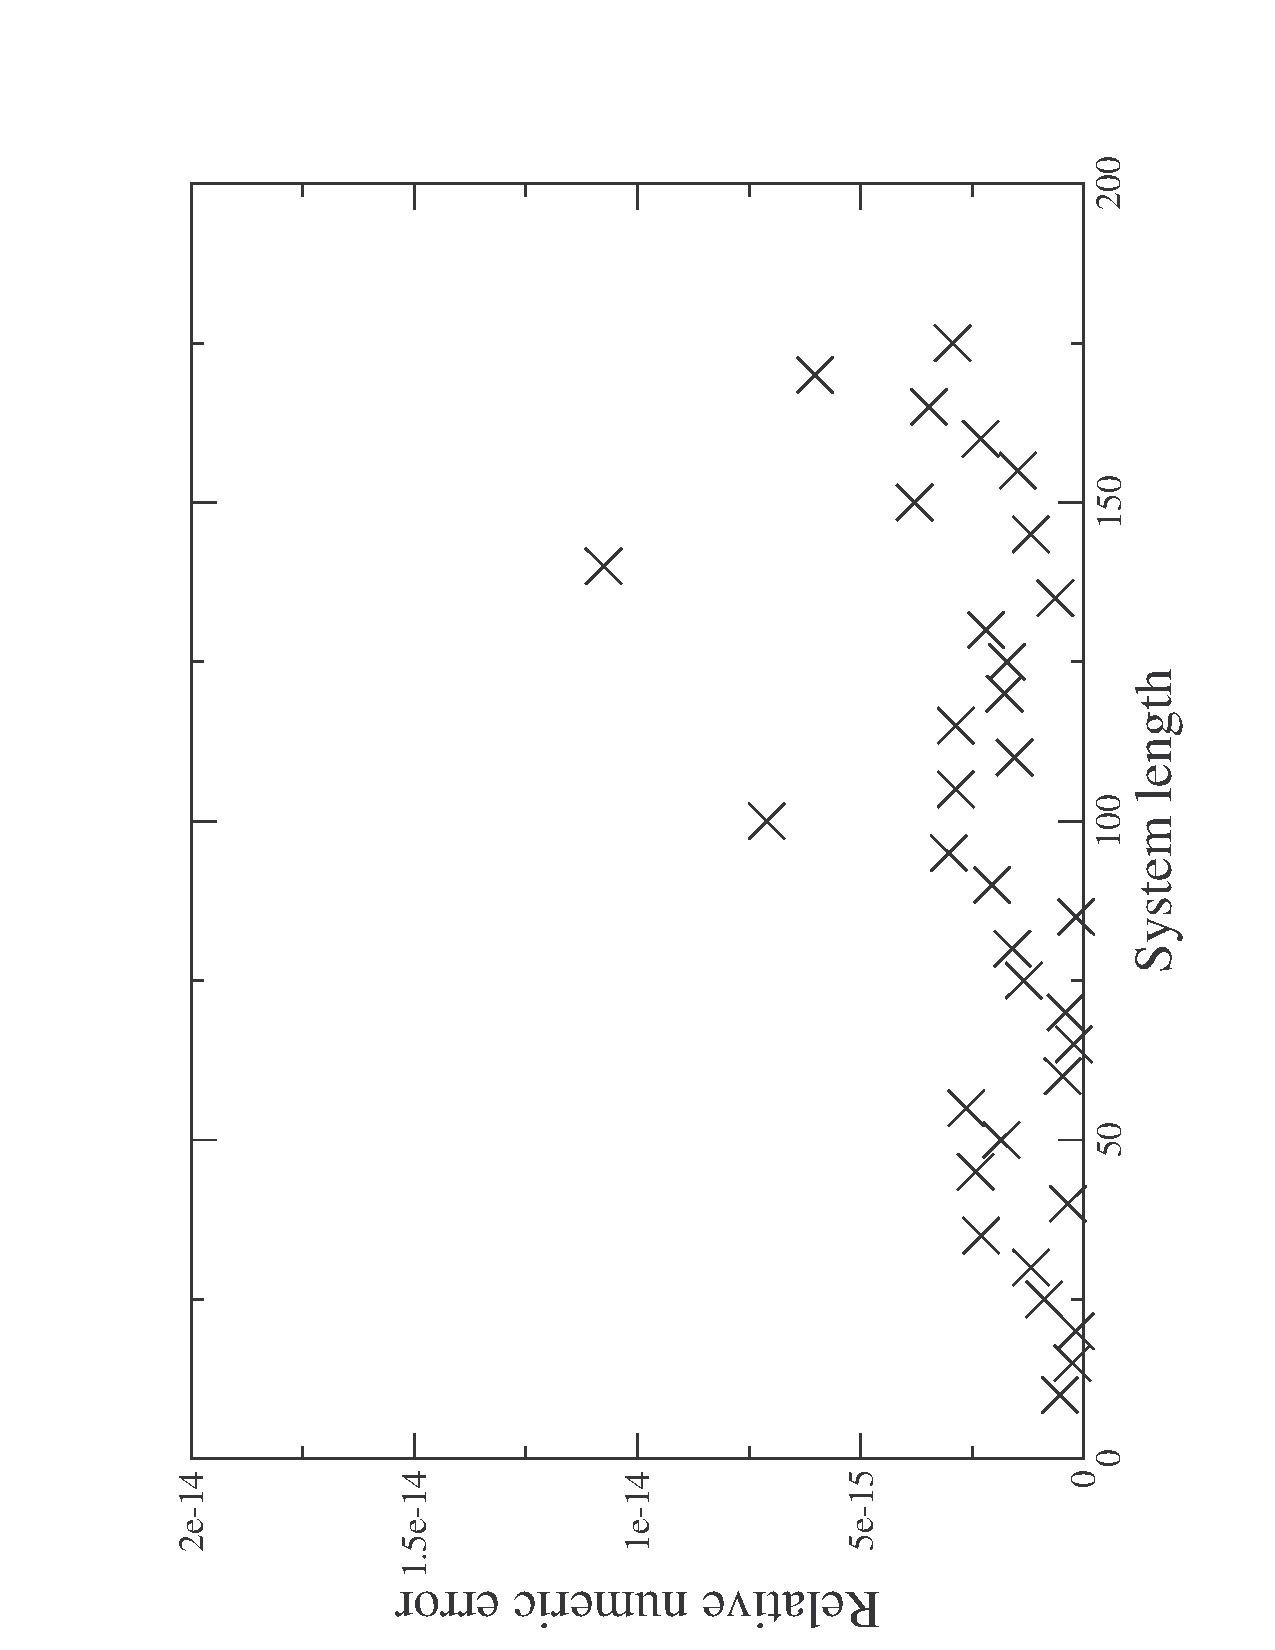
\includegraphics[angle=270,width=0.7\textwidth]{numeric-errors.pdf}
    \caption{Numerical errors in $T_{pq}$ as a function of system size.}
    \label{fig:numeric-errors}
\end{figure}

Fig. \ref{fig:numeric-errors} shows the estimate of the numerical errors, and
that they are well below $10^{-13}$ for the investigated systems, and are
thusly no source for worries.

\section{Quality checks}

Programming is constantly prone to subtle errors, so measures had to 
be taken to ensure that no errors slipped in that might lead to wrong
output.

The program discussed herein is basically a function that constructs a
Hamilton operator from the Rashba coupling strength, magnetic
field and other parameters, and then calculates the transmission
matrix $T_{pq}$ from that Hamilton operator.

The very first sanity check is that $H$ is indeed a hermitian
operator. This check of course only catches stupid programming
mistakes.

A more elaborate check is that $T_{pq}$ obeys the same symmetries as
the Hamiltonian. Since it can be written as
  
\begin{equation}
H = \frac{\vec{p}^2}{2 m^*} + \vec \sigma \cdot (\vec e_z \times \vec p)  
    + \vec \sigma \cdot \vec B
\end{equation}

It is easy to see that $H(\vec p, \vec \sigma, \vec B) = H(-\vec p,
-\vec \sigma, -\vec B)$, so the transmission matrix must follow the
same symmetries.

We checked these symmetries and the sum rule (eq. \ref{eq:sumrule}) regularly
to ensure that no simple errors slipped in.

\section{Setup}

\begin{figure}
    \begin{center}
        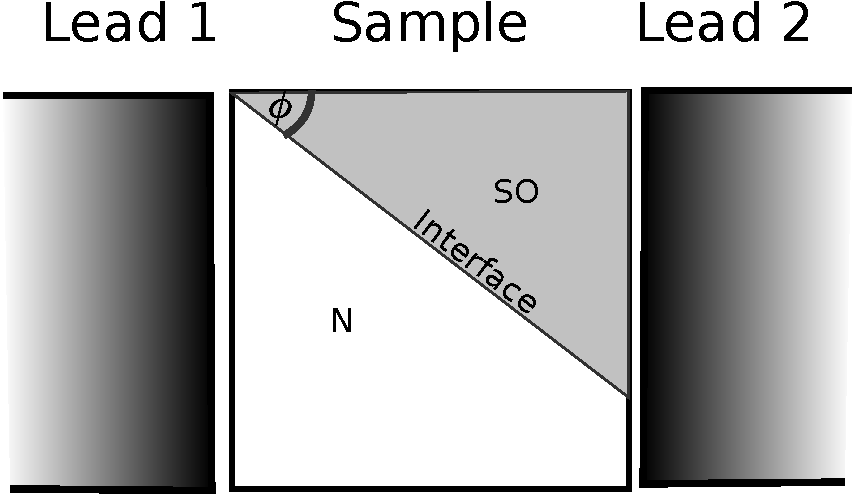
\includegraphics[width=0.5\textwidth]{sample-lead-interface.pdf}%
        \hspace{0.1\textwidth}%
        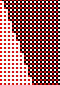
\includegraphics[width=0.2\textwidth]{hopping.png}
    \end{center}
    \caption{\textbf{Left:} the sample is connected to one lead for each spin
        on the left and on the right.
        \textbf{Right:}
        Detail from an interface between normal and spin-orbit coupling regime modeled
        in the tight binding model, at angle $\phi = 70\,^{\circ}$.
        Red dots show lattice sites, black dots
        show non-zero hopping elements with spin flips.}
    \label{fig:interface-setup}
\end{figure}

For the following simulations we used a square sample, typically of $100
\times 100$ lattice sites, with two leads attached both on the left and on the
right, on for spin up, one for spin down.

To simulate an interface of an arbitrary angle $\phi$, we calculate the Rashba
hopping elements separately for each lattice sites, and install them for
hopping to the right and upper neighbor each. Fig. \ref{fig:interface-setup}
shows how such an interface looks.

\begin{figure}
    \begin{center}
        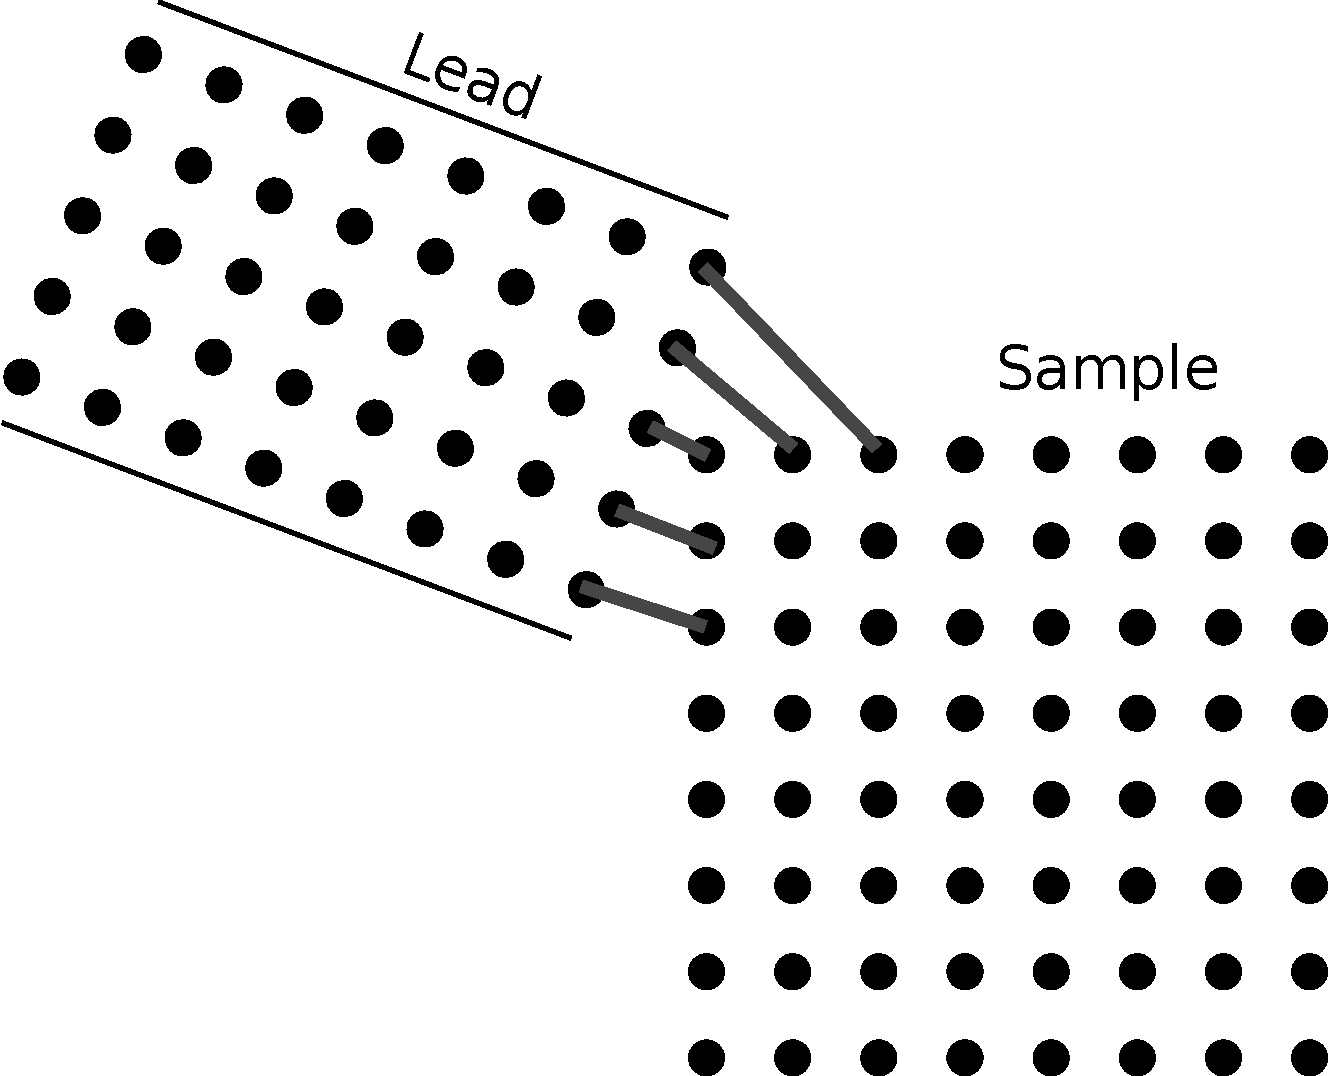
\includegraphics[width=0.4\textwidth]{lead-tilted-1.pdf}
        \hspace{0.1\textwidth}
        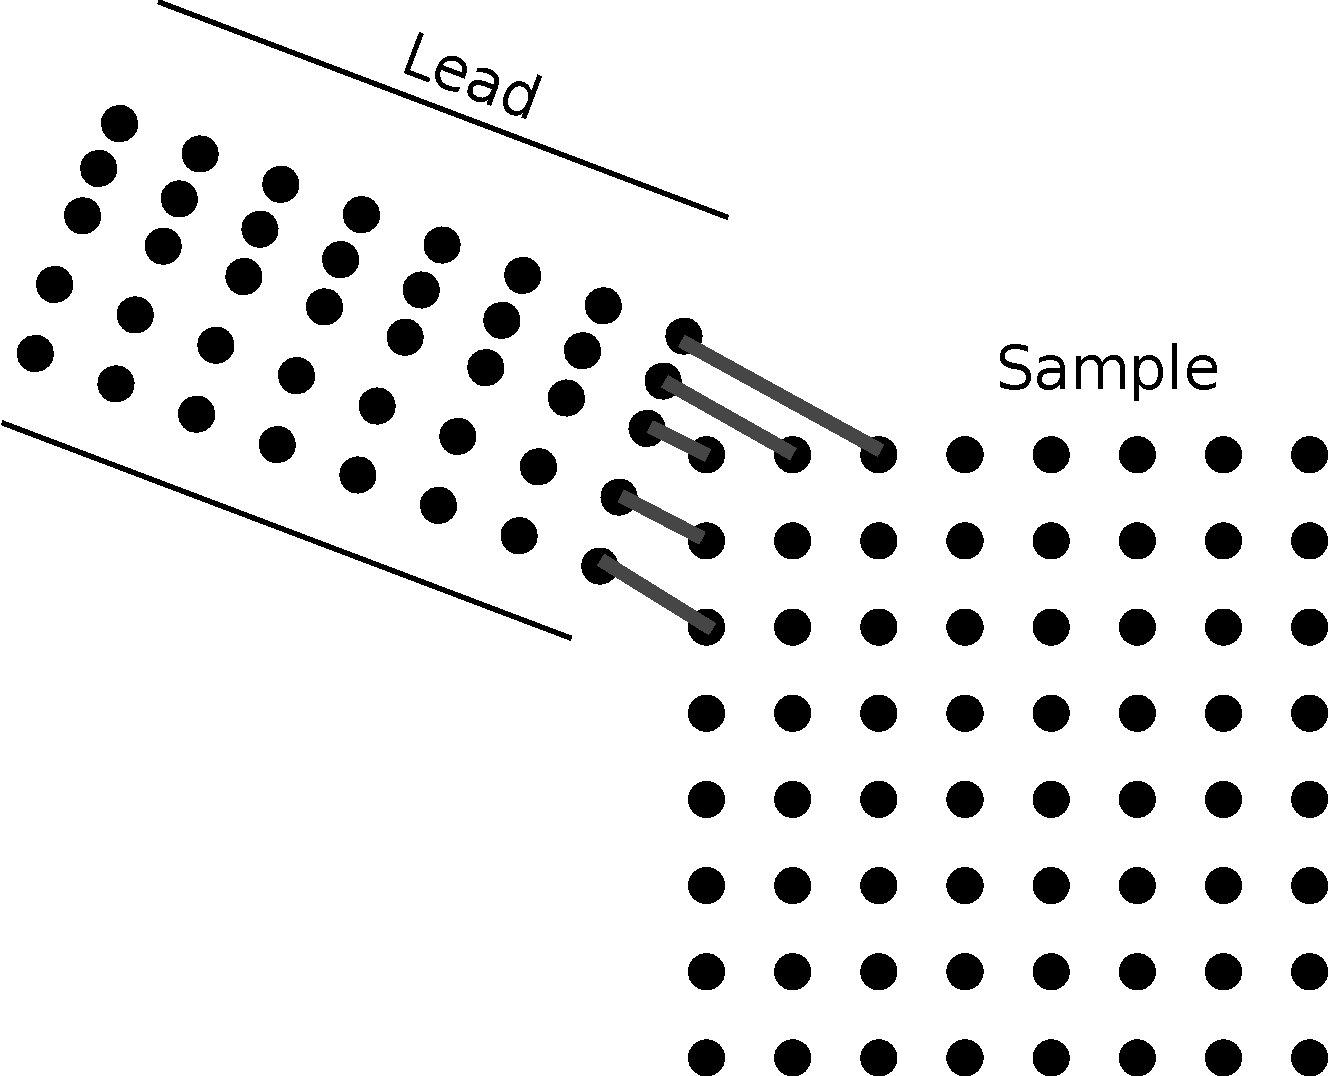
\includegraphics[width=0.4\textwidth]{lead-tilted-2.pdf}
    \end{center}
    \caption{Two ways to attach a tilted lead. \textbf{Left:} equal lattice
        spacing in lead and sample. \textbf{Right:} parallel projection from
        the sample into the lead leads to uneven lattice spacing in the lead.}
    \label{fig:tilted-leads}
\end{figure}

To obtain a smoother interface we also experimented with using a vertical
interface, and
injecting the electron beam with a tilted lead. There are two possible
ways to do this (as illustrated by figure \ref{fig:tilted-leads}):
either one can assume the same lattice spacing in lead and sample, and assume
coupling even though the geometry doesn't match, or one can project the sites
from the edge of the sample parallel into the lead, and then get a non-regular
lattice spacing in the lead.

The former turned out not to work the way we wanted it to: instead of one
electron beam propagating in the same direction as the lead, there were two
beams, one parallel to each side of the edge of the sample. The latter is
physically hard to interpret and also much effort to implemented, so we set
that idea aside.

\section{Interface between normal and spin-orbit coupling region}

\begin{figure}
    \begin{center}
    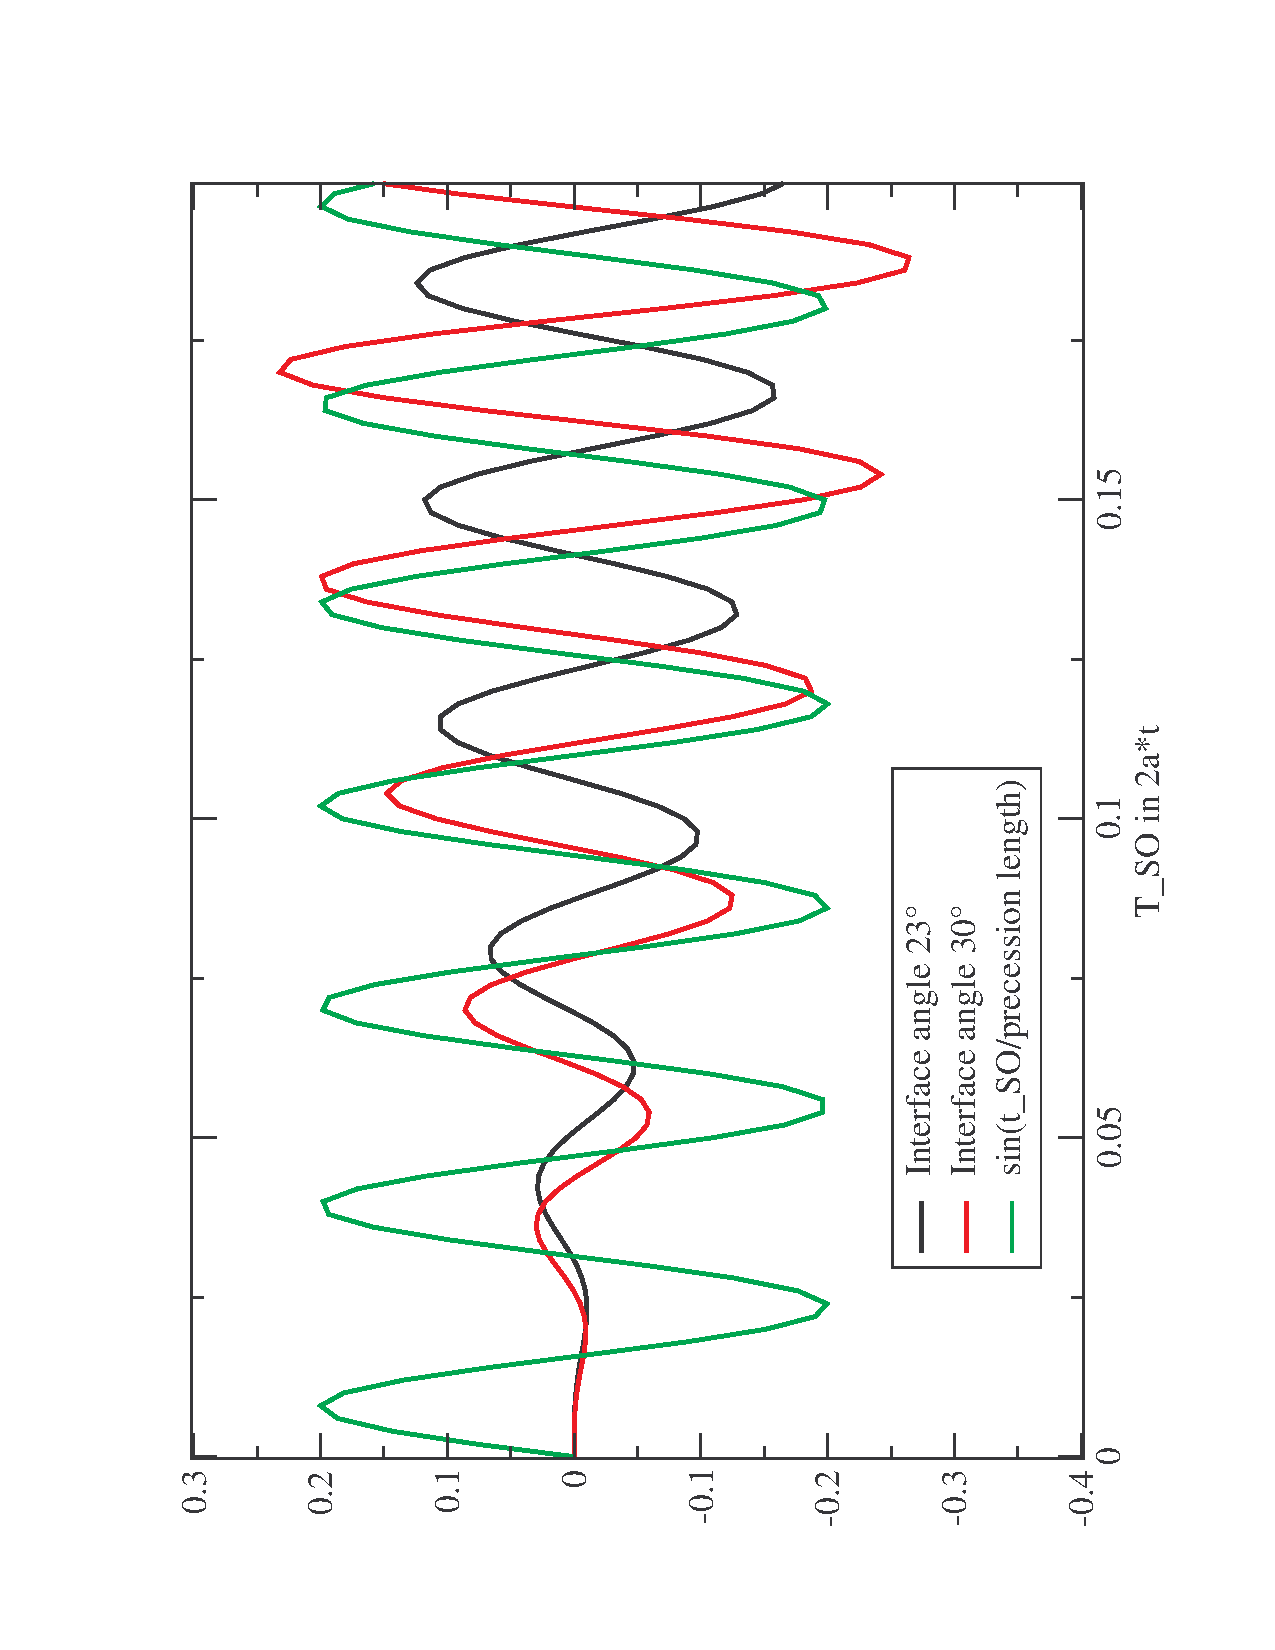
\includegraphics[angle=270,width=0.7\textwidth]{interface-precession.pdf}
    \end{center}
    \caption{$T_S = T_{2\uparrow,1\uparrow}-T_{2\downarrow,1\downarrow}$ as a
        function of spin orbit coupling strength. The interface causes a
        separation of spins, which oscillates and is dependent on the angle of
        the interface.}
    \label{fig:interface-precession}
\end{figure}

When plotting $T_S = T_{2\uparrow,1\uparrow}-T_{2\downarrow,1\downarrow}$ as a
function of spin orbit coupling strength, one sees that the signal oscillates
(see figure \ref{fig:interface-precession}).
This is caused by the well-known % TODO: cite
spin precession: in a medium with spin-orbit coupling $\sigma_z$ is not a good
quantum number anymore, and the spin precesses. % around what?

So if an electron is injected with spin up, and is measured after the
precession length $\lso = \frac{t}{\tso}\pi a$ it is again found to have
spin up, but after $\frac12 \lso$ or $\frac32 \lso$ the spin points
downwards. 

Since  $\lso$ is a function of $\tso$, the precession can also be
observed when $\tso$ is varied (and not the width of the sample).
If $n$ is an integer and $W$ with width of our sample, we should see the
same signal for $W = n \cdot \lso(n)$ and $W = (n+1) \lso(n+1)$. So
$\tso(n) = n\frac{\pi t}{W}$, and $\Delta \tso = \frac{\pi t}{W}$.  The green
curve in figure \ref{fig:interface-precession} shows the curve
$\sin{\frac{2 \pi \tso}{\Delta \tso}}$, and thus the expected spin precession.

Only a part of the sample has non-zero spin-orbit coupling strength, so $T_S$
actually precesses with a slightly longer period than $\Delta \tso$.

\subsection{Comparison to analytical results}

The chiral spin bases as introduced in chapter \ref{sec:analytica} are very
natural for the analytical calculation, because the
base vectors are also eigenstates to the Hamiltonian.

However for the numerical simulation they are not suited, because they are
dependent on the direction (in real space) in which the wave travels. This
is not known before the simulation runs, and because there can be several
waves with different directions in one place, it is not possible to calculate
the self-energy of the leads in these bases.

\begin{figure}
    \begin{center}
    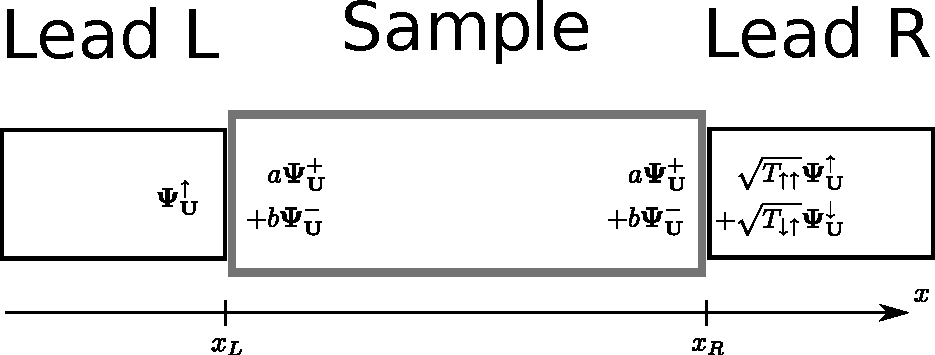
\includegraphics[width=0.8\textwidth]{adapting-pic.pdf}
    \end{center}
    \caption{Injecting one spin-up charge carrier into the system}
\end{figure}

% Since there is no dissipation in our model, and we assume that the mere
% process of injecting an electron doesn't change its spin, we can project
% the $|\uparrow>$ and $|\downarrow>$ states separately onto the wave
% function in the sample:

Since we assume that our leads are perfect semi-infinite wires, we can assume
that the wave functions are plain waves

\begin{align*}
    \mathbf{\Psi^\uparrow}   &=  e^{i p_x x} e^{i p_z z} |\uparrow> \\
    \mathbf{\Psi^\downarrow} &=  e^{i p_x x} e^{i p_z z} |\downarrow> \\
\end{align*}

and that the wave functions are continuous at the interface:

\begin{align*}
    \mathbf{\Psi^\uparrow}(x=x_1) &=
        a \mathbf{\Psi^+_U}(x=x_1) + b  \mathbf{\Psi^-_U}(x=x_1)\\
    \mathbf{\Psi^\downarrow}(x=x_1) &=
        c \mathbf{\Psi^+_U}(x=x_1) + d  \mathbf{\Psi^-_U}(x=x_1)
\end{align*}

Where $x_1$ is the location where the left lead is connected to the sample, the
interface is at $x = 0$ and the right lead is connected at $x = x_2$.
Each of these equations has two components, which allows us to determine
$a, b, c$ and $d$ unambiguously.

With $\mathbf{\Psi^\pm_U}$ we mean the wave function normalized to 1 at the
left hand side of the interface, so for example
$|\mathbf{\Psi^\pm_U}(x=x_1)|=1$. For $x>0$ the amplitude of the wave function
is smaller than 1, due to reflection at the interface.

We can then look at the connection to the right lead, and obtain the 
elements of the transmission matrix in the $\uparrow, \downarrow$ bases:

\begin{align}
    T_{2\uparrow,1\uparrow} = \left| \left( 
        a \mathbf{\Psi^+_U}(x=x_2) + b  \mathbf{\Psi^-_U}(x=x_2)
    \right)^\dagger \cdot \mathbf{\Psi}^\uparrow(x=x_2) \right|^2\\
    T_{2\downarrow,1\uparrow} = \left| \left( 
        a \mathbf{\Psi^+_U}(x=x_2) + b  \mathbf{\Psi^-_U}(x=x_2)
    \right)^\dagger \cdot \mathbf{\Psi}^\downarrow(x=x_2) \right|^2\\
    T_{2\uparrow,1\downarrow} = \left| \left( 
        c \mathbf{\Psi^+_U}(x=x_2) + d  \mathbf{\Psi^-_U}(x=x_2)
    \right)^\dagger \cdot \mathbf{\Psi}^\uparrow(x=x_2) \right|^2\\
    T_{2\downarrow,1\downarrow} = \left| \left( 
        c \mathbf{\Psi^+_U}(x=x_2) + d  \mathbf{\Psi^-_U}(x=x_2)
    \right)^\dagger \cdot \mathbf{\Psi}^\downarrow(x=x_2) \right|^2
\end{align}

Since the analytical model looks at a single mode, but the numerical
calculation allows one mode per spin-dependent lead (and thus two modes in
sum) to propagate, we have to multiply the results from the analytical
calculation by a factor of 2 when comparing with results from the numerical
simulation.

\begin{figure}
    \begin{center}
        \includegraphics[width=0.8\textwidth]{a-n-matching-over-alpha.pdf}
    \end{center}
    \caption{$T_S = T_{2\uparrow,1\uparrow} - T_{2\downarrow,2\downarrow}$ as
        a function of $\ta$. Bold curves show the results from the analytical
        calculations, thin lines from the numerical calculation.
        \textbf{Blue:} $\phi = 23^\circ$, \textbf{Red:} $\phi = 29^\circ$.
    }
    \label{fig:a-n-matching-alpha}
\end{figure}

Figure \ref{fig:a-n-matching-alpha} shows the signal for two different
angles of the interface. For weak spin-orbit coupling the theory and the
numerical results agree well, for stronger coupling both the oscillation
period and the amplitude start to disagree.


% vim: ts=4 sw=4 expandtab spell spelllang=en_us tw=78
